\documentclass{article}
\usepackage[14pt]{extsizes}
\usepackage[utf8]{inputenc}
\usepackage{amsmath}
\usepackage{amsfonts}
\usepackage{amssymb}
\usepackage{tabularx}
\usepackage{multirow}
\newcommand{\RomanNumeralCaps}[1]
{\MakeUppercase{\romannumeral #1}}
\usepackage{cmap} % для кодировки шрифтов в pdf
\usepackage[T2A]{fontenc}
\usepackage[russian]{babel}
\usepackage{graphicx} % для вставки картинок
\usepackage{amssymb,amsfonts,amsmath,amsthm} % математические дополнения от АМС
\usepackage{indentfirst} % отделять первую строку раздела абзацным отступом тоже

\usepackage{listings}
\usepackage{color} %red, green, blue, yellow, cyan, magenta, black, white
\definecolor{mygreen}{RGB}{28,172,0} % color values Red, Green, Blue
\definecolor{mylilas}{RGB}{170,55,241}
% Поля
\usepackage{geometry}
\geometry{left=3cm}
\geometry{right=1.5cm}
\geometry{top=2.4cm}
\geometry{bottom=2.cm}

%%%%%%%%%%%%%%%%%%%%%%%%%%%%%%%    

\linespread{1.5} % полуторный интервал
\renewcommand{\rmdefault}{ftm} % Times New Roman
\frenchspacing

% подключаем hyperref (для ссылок внутри  pdf)
\usepackage[unicode, pdftex]{hyperref}

% коррекция подрисуночной подписи
\usepackage{caption}
\captionsetup[figure]{labelsep=period} %Точка
%\captionsetup[figure]{labelsep=space}  %Пробел
%\captionsetup[figure]{labelsep=endash}  %Новый страндарт
\usepackage[figurename=Рисунок]{caption}

     \graphicspath{{../der}}

\begin{document}
	
	\begin{titlepage}
		
		\begin{center}
			САНКТ-ПЕТЕРБУРГСКИЙ ГОСУДАРСТВЕННЫЙ ЭЛЕКТРОТЕХНИЧЕСКИЙ УНИВЕРСИТЕТ «ЛЭТИ» \\ИМ. В.И. УЛЬЯНОВА (ЛЕНИНА)\\
			\vspace{0.1cm}
			Кафедра Алгоритмической математики\\
			
			
			
		\end{center}
		
		\vspace{5cm}
		\begin{center}
			\begin{large}
				Лабораторная работа 1 \\
				"Интерполяция"
			\end{large}
		\end{center}
		
		\vspace{5cm}
		
		\hspace{5cm} Студент гр.  0307 \hrulefill Латин Я.М.
		
		\vspace{0.5cm}
		\hspace{5cm} Преподаватель \hrulefill  Солнышкин С.Н.\\
		
		
		\vfill
		\begin{center}
			Санкт-Петербург\\
			2022
		\end{center}
		
		
	\end{titlepage}
	
	
	\newpage
	\tableofcontents
	\newpage
	
	\section{Цель работы}
	Построение интерполяционного многочлена по равноотстоящим и чебышёвским узлам. Нахождение  фактической и теоретической погрешности.
	\section{Задание}
	Построить интерполяционный многочлен по 2, 3, 4, 5 и 6 узлам (равноотстоящим и чебышёвским) для функции $f(x)=\frac{1000}{\sqrt{x^2-5x+60}}$, на промежутке $[a; b] = [-1; 7]$ по равноотстоящим и по чебышёвским узлам. Найти фактическую погрешность и сравнить нё с теоретической оценкой.
	  
	\section{Построение интерполяционного многочлена по равноотстоящим узлам}
	
	\subsection{Интерполяционные многочлены}
	\begin{flushleft}
		$ L_1(x)=-0.2047502048 x+14.9467649468 $\\
		$ L_2(x)=-0.2616252616 x^2+1.3650013650 x+16.7781417781 $\\
		$L_3(x)=0.0082165104x^3-0.3274970826x^2+1.4069223421x+ 16.8941510867$\\
		$L_4(x)= 0.0043773481x^4-0.0447891072x^3-0.1649376649x^2  +$\\
		$1.3976029601x+16.6648893211$\\
		$L_5(x)=-0.0002123162x^5+0.0073916032x^4-0.0575766822x^3 -0.1522933884x^2+1.4134028413x+16.6520307796$
	\end{flushleft}

	\newpage
	
	\subsection{Графики интерполяционных многочленов:}
	
	\begin{figure}[h]
		\begin{minipage}[h]{0.47\linewidth}
			\center{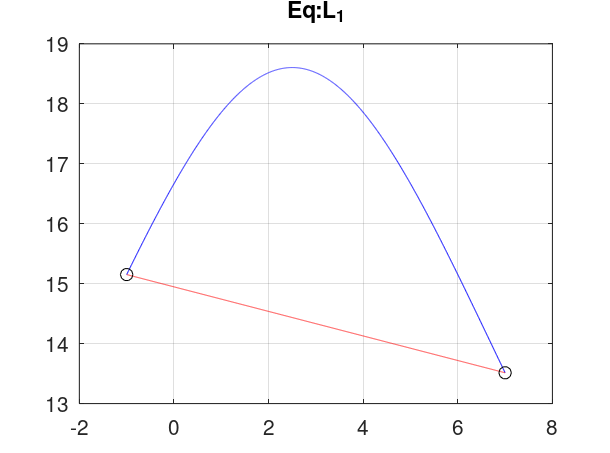
\includegraphics[width=1\linewidth]{../polinom degree/eq/eq1}}  \\
		\end{minipage}
		\hfill
		\begin{minipage}[h]{0.47\linewidth}
			\center{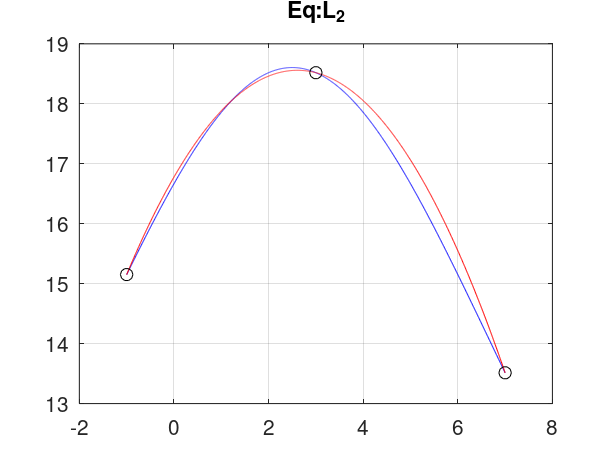
\includegraphics[width=1\linewidth]{../polinom degree/eq/eq2}} \\
		\end{minipage}
		\vfill
		\begin{minipage}[h]{0.47\linewidth}
			\center{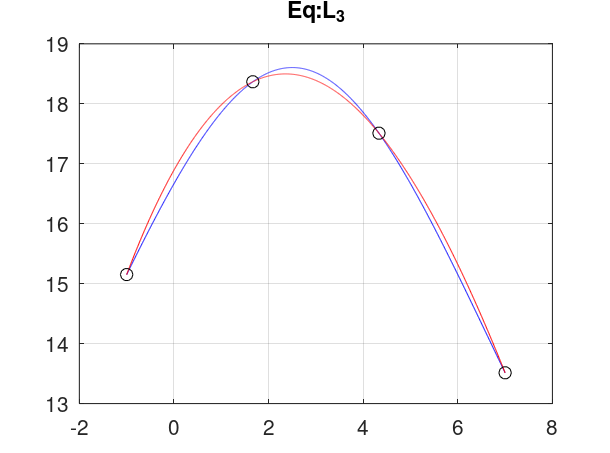
\includegraphics[width=1\linewidth]{../polinom degree/eq/eq3}}  \\
		\end{minipage}
		\hfill
		\begin{minipage}[h]{0.47\linewidth}
			\center{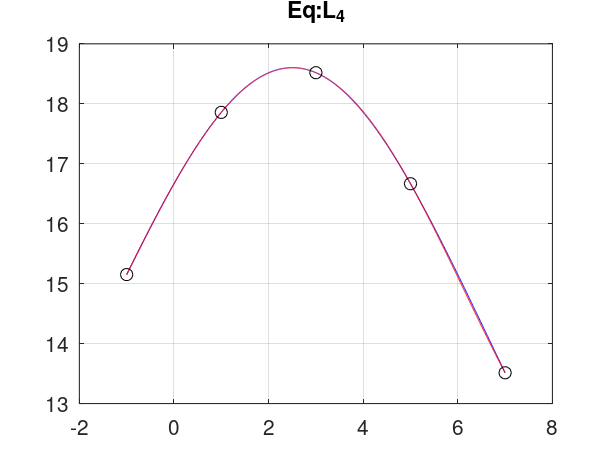
\includegraphics[width=1\linewidth]{../polinom degree/eq/eq4}}  \\
		\end{minipage}
		\vfill
		\begin{minipage}[h]{0.47\linewidth}
			\center{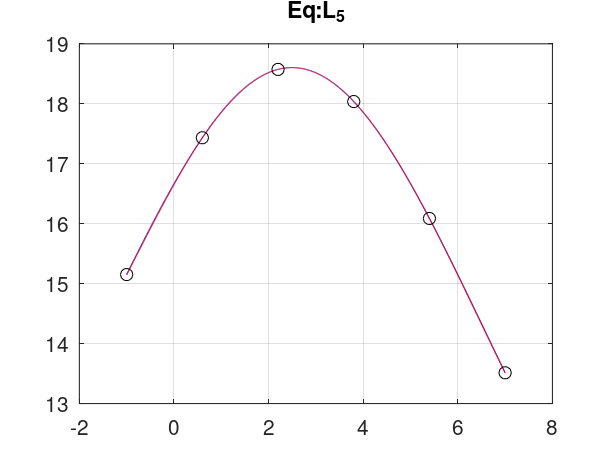
\includegraphics[width=1\linewidth]{../polinom degree/eq/eq5}}  \\
		\end{minipage}
	\end{figure}
	\newpage
	\subsection{Графики погрешностей}
	\begin{figure}[h]
		\begin{minipage}[h]{0.47\linewidth}
			\center{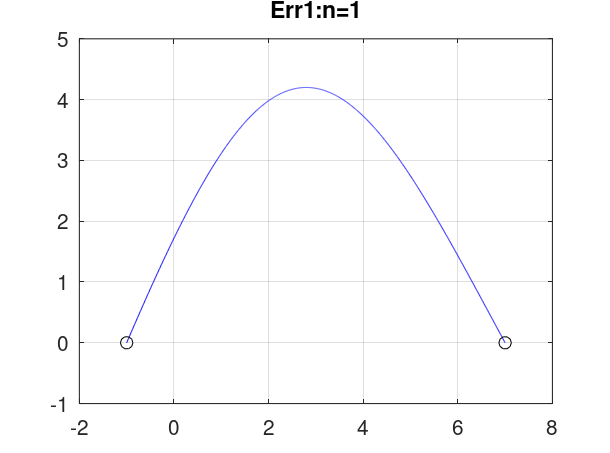
\includegraphics[width=1\linewidth]{../polinom degree/err/err1}}  \\
		\end{minipage}
		\hfill
		\begin{minipage}[h]{0.47\linewidth}
			\center{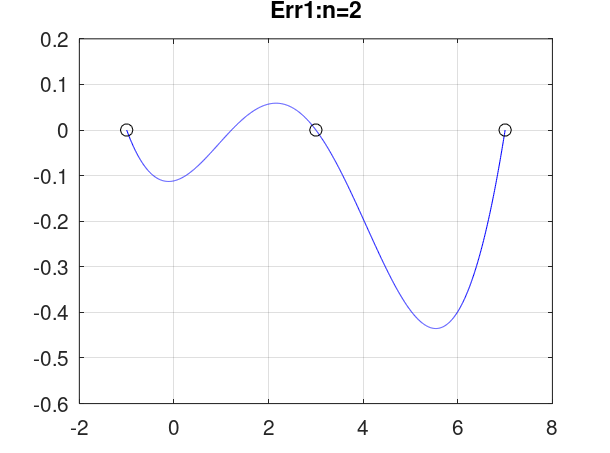
\includegraphics[width=1\linewidth]{../polinom degree/err/err2}} \\
		\end{minipage}
		\vfill
		\begin{minipage}[h]{0.47\linewidth}
			\center{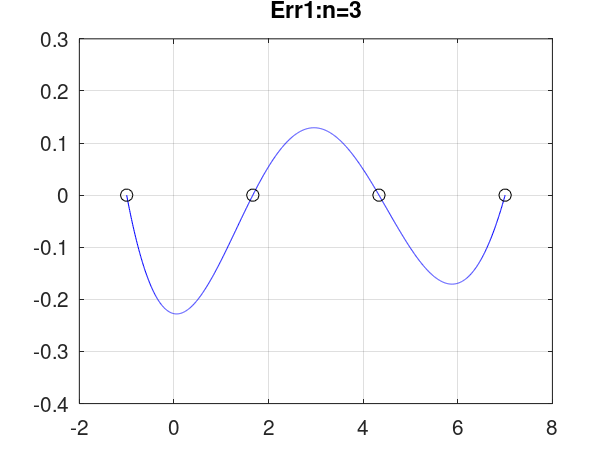
\includegraphics[width=1\linewidth]{../polinom degree/err/err3}}  \\
		\end{minipage}
		\hfill
		\begin{minipage}[h]{0.47\linewidth}
			\center{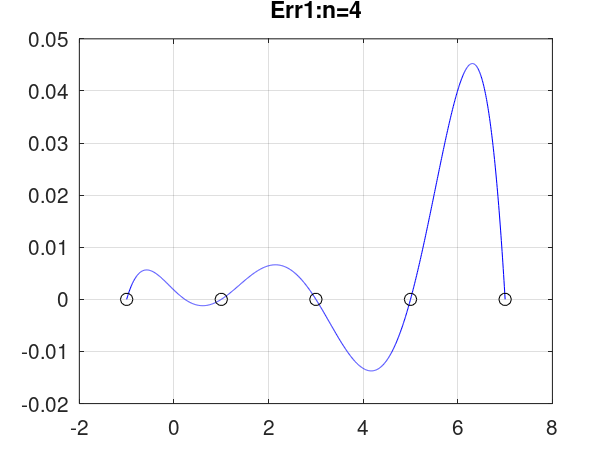
\includegraphics[width=1\linewidth]{../polinom degree/err/err4}}  \\
		\end{minipage}
		\vfill
		\begin{minipage}[h]{0.47\linewidth}
			\center{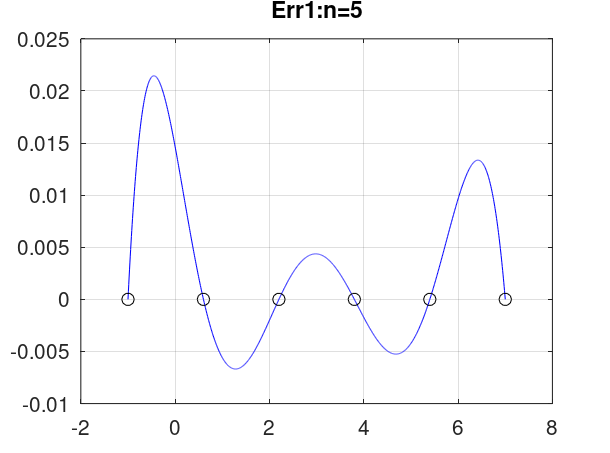
\includegraphics[width=1\linewidth]{../polinom degree/err/err5}}  \\
		\end{minipage}
	\end{figure}
	
	\newpage
	
	\section{Построение интерполяционного многочлена по чебышёвским узлам}
		\subsection{Интерполяционные многочлены}
			\begin{flushleft}
				$ L_1(x)=-0.2606882169 x+16.9447340980 $\\
				$ L_2(x)=-0.2770956960 x^2+1.4323715981 x+16.7152649887 $\\
				$L_3(x)=0.0084960616x^3-0.3360434158x^2+1.4517213711x+ 16.8095616750$\\
				$L_4(x)= 0.0043618026x^4-0.0446617233x^3-0.1640351345x^2  +$\\
				$1.3939066976x+16.6656751544$\\
				$L_5(x)=-0.0002041496x^5+0.0071536259x^4-0.0556377472x^3 -0.1564960714x^2+1.4090036379x+16.6631419171$
			\end{flushleft}
		\newpage
		\subsection{Графики интерполяционных многочленов:}
			\begin{figure}[h]
				\begin{minipage}[h]{0.47\linewidth}
					\center{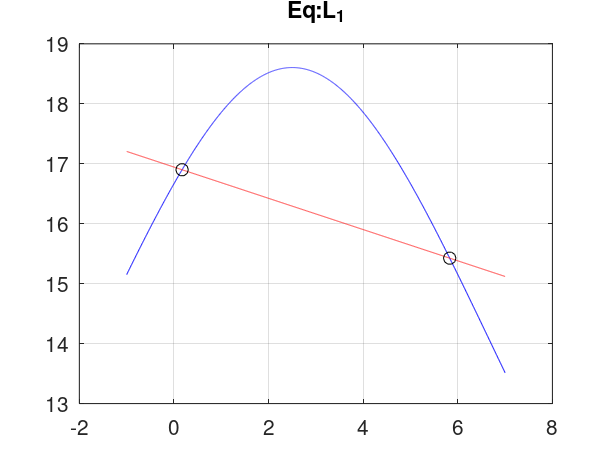
\includegraphics[width=1\linewidth]{../Chebyshev/eq/eq1}}  \\
				\end{minipage}
				\hfill
				\begin{minipage}[h]{0.47\linewidth}
					\center{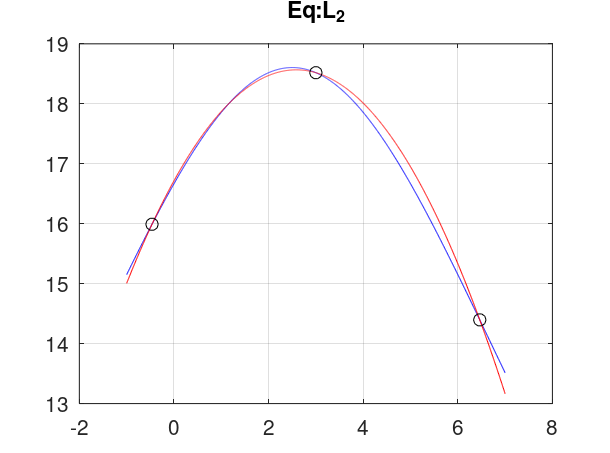
\includegraphics[width=1\linewidth]{../Chebyshev/eq/eq2}} \\
				\end{minipage}
				\vfill
				\begin{minipage}[h]{0.47\linewidth}
					\center{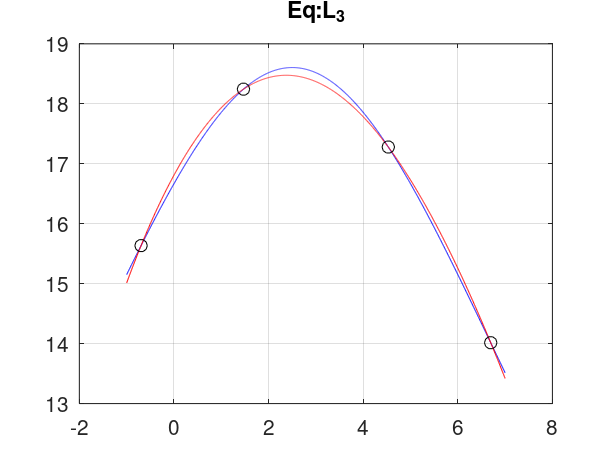
\includegraphics[width=1\linewidth]{../Chebyshev/eq/eq3}}  \\
				\end{minipage}
				\hfill
				\begin{minipage}[h]{0.47\linewidth}
					\center{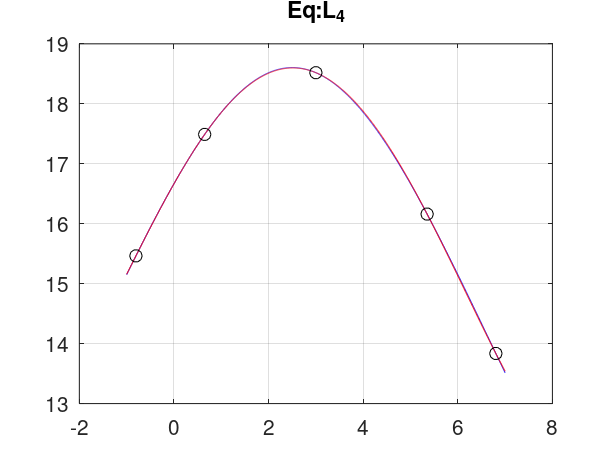
\includegraphics[width=1\linewidth]{../Chebyshev/eq/eq4}}  \\
				\end{minipage}
				\vfill
				\begin{minipage}[h]{0.47\linewidth}
					\center{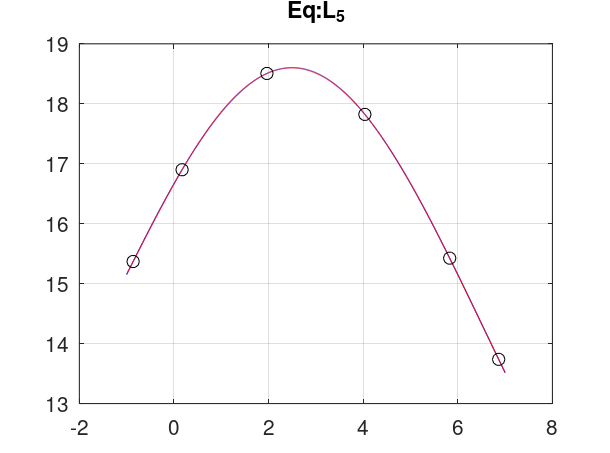
\includegraphics[width=1\linewidth]{../Chebyshev/eq/eq5}}  \\
				\end{minipage}
			\end{figure}
		\newpage
		\subsection{Графики погрешностей:}
			\begin{figure}[h]
				\begin{minipage}[h]{0.47\linewidth}
					\center{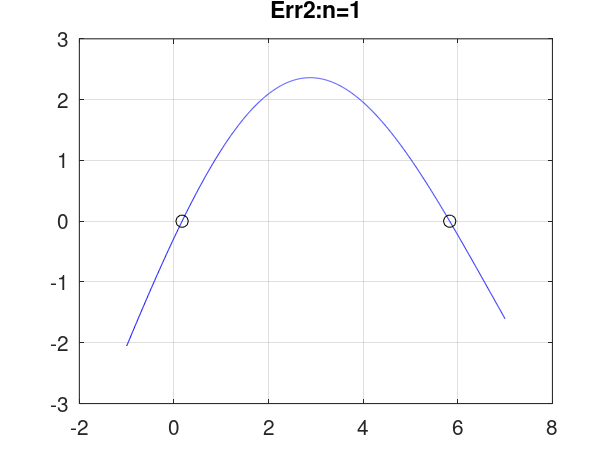
\includegraphics[width=1\linewidth]{../Chebyshev/err/err1}}  \\
				\end{minipage}
				\hfill
				\begin{minipage}[h]{0.47\linewidth}
					\center{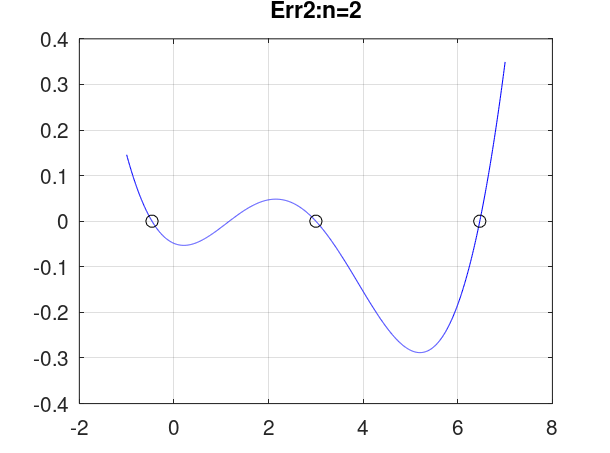
\includegraphics[width=1\linewidth]{../Chebyshev/err/err2}} \\
				\end{minipage}
				\vfill
				\begin{minipage}[h]{0.47\linewidth}
					\center{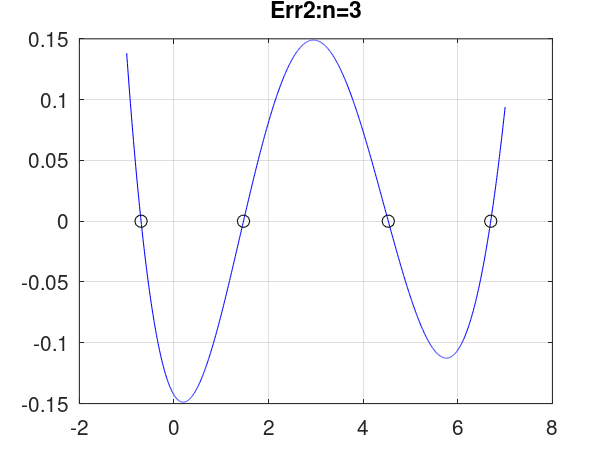
\includegraphics[width=1\linewidth]{../Chebyshev/err/err3}}  \\
				\end{minipage}
				\hfill
				\begin{minipage}[h]{0.47\linewidth}
					\center{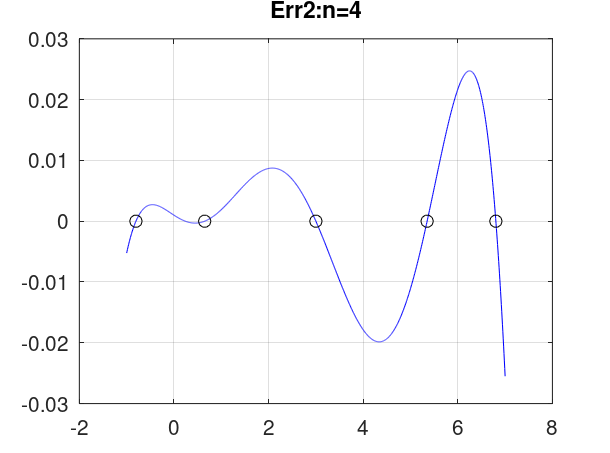
\includegraphics[width=1\linewidth]{../Chebyshev/err/err4}}  \\
				\end{minipage}
				\vfill
				\begin{minipage}[h]{0.47\linewidth}
					\center{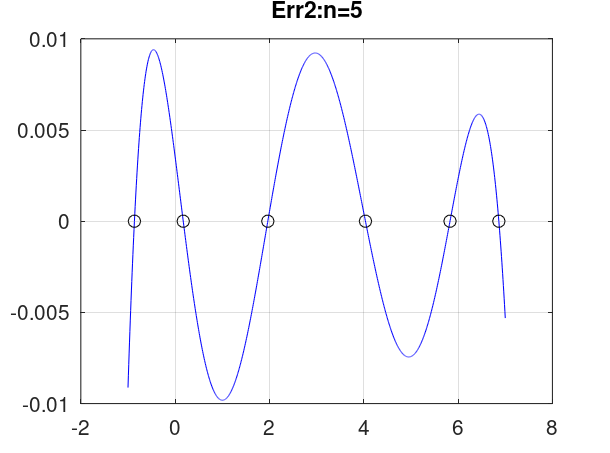
\includegraphics[width=1\linewidth]{../Chebyshev/err/err5}}  \\
				\end{minipage}
			\end{figure}
	\newpage
	\section{Графики производных}
		\begin{figure}[h]
			\begin{minipage}[h]{0.47\linewidth}
				\center{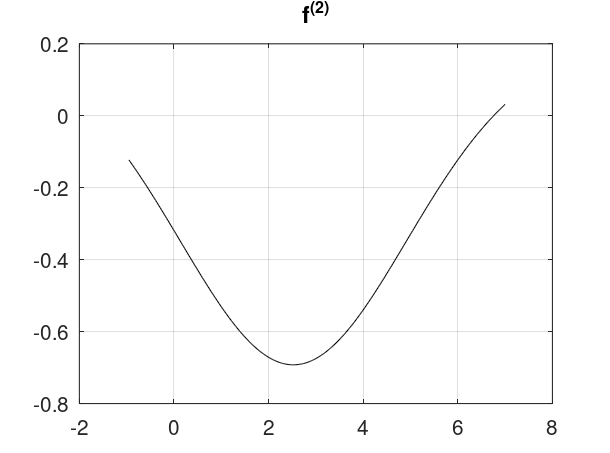
\includegraphics[width=1\linewidth]{2}}  \\
			\end{minipage}
			\hfill
			\begin{minipage}[h]{0.47\linewidth}
				\center{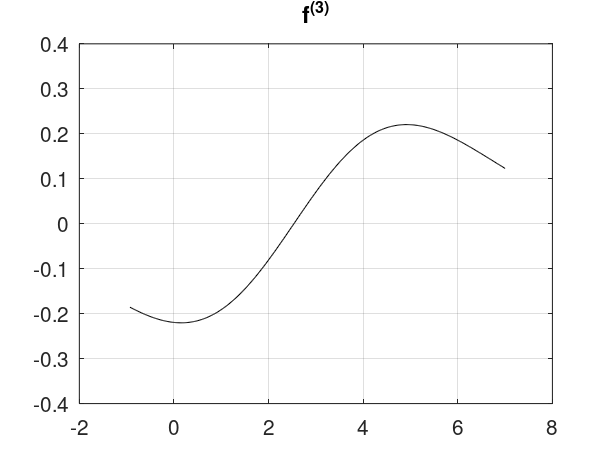
\includegraphics[width=1\linewidth]{3}} \\
			\end{minipage}
			\vfill
			\begin{minipage}[h]{0.47\linewidth}
				\center{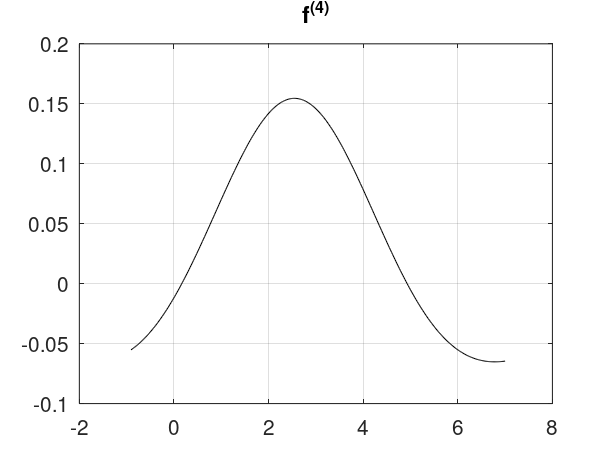
\includegraphics[width=1\linewidth]{4}}  \\
			\end{minipage}
			\hfill
			\begin{minipage}[h]{0.47\linewidth}
				\center{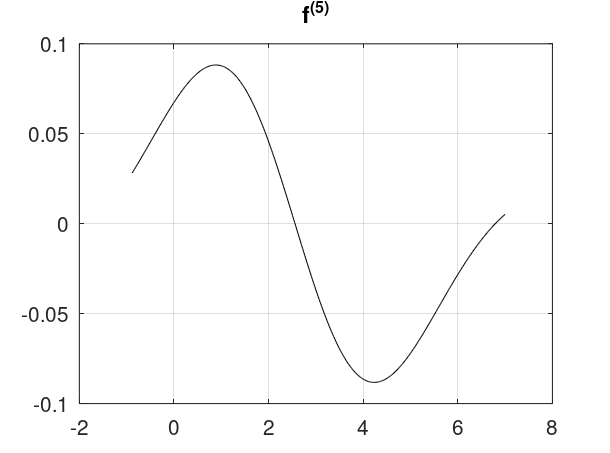
\includegraphics[width=1\linewidth]{5}}  \\
			\end{minipage}
			\vfill
			\begin{minipage}[h]{0.47\linewidth}
				\center{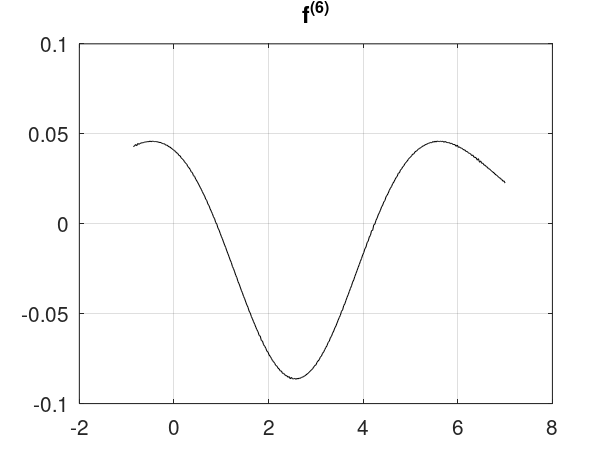
\includegraphics[width=1\linewidth]{6}}  \\
			\end{minipage}
		\end{figure}
	\newpage
	
	\section{Оценка погрешностей}
	\begin{flushright}
		Таблица 1. Равноотстоящие узлы
	\end{flushright}
	\begin{table}[!h]
		\centering
		\begin{tabular}{|c|c|c|c|c|c|}
			\hline
			$n$              & 1       & 2       & 3       & 4        & 5        \\ \hline
			$(n+1)!$         & 2       & 6       & 24      & 120      & 720      \\ \hline
			$max|\omega_{n+1}|$   & 16      & 24.634  & 50.568  & 116.21   & 283.55   \\ \hline
			$max|f^{(n+1)}|$ & 0.69226 & 0.22041 & 0.15454 & 0.088228 & 0.086487 \\ \hline
			$R_\text{факт}$              & 4.2001 &    0.43542     &    0.22798     &     0.04526     &     0.021455     \\ \hline
			$R_\text{теор}$              &   5.53808      &     0.90493     &   0.325616      &    0.0854415       &    0.0340603      \\ \hline
		\end{tabular}
	\end{table}
\begin{flushright}
	Таблица 2. Чебышёвские узлы
\end{flushright}
\begin{table}[!h]
	\centering
	\begin{tabular}{|c|c|c|c|c|c|}
		\hline
		$n$              & 1       & 2       & 3       & 4        & 5        \\ \hline
		$(n+1)!$         & 2       & 6       & 24      & 120      & 720      \\ \hline
		$max|\omega_{n+1}|$   & 8      & 16  & 32  & 64   & 128  \\ \hline
		$max|f^{(n+1)}|$ & 0.69226 & 0.22041 & 0.15454 & 0.088228 & 0.086487 \\ \hline
		$R_\text{факт}$              & 2.3609 &    0.34934     &    0.14899     &     0.025504     &     0.0098184     \\ \hline
		$R_\text{теор}$     &  2.76904  &  0.58776   &  0.206053    &   0.0470549  &   0.0153755   \\ \hline
	\end{tabular}
\end{table}
	
	\newpage
	\section{Код сценариев и функции}
	\lstset{language=Matlab,%
		%basicstyle=\color{red},
		breaklines=true,%
		morekeywords={matlab2tikz},
		keywordstyle=\color{blue},%
		morekeywords=[2]{1}, keywordstyle=[2]{\color{black}},
		identifierstyle=\color{black},%
		stringstyle=\color{mylilas},
		commentstyle=\color{mygreen},%
		showstringspaces=false,%without this there will be a symbol in the places where there is a space
		numbers=left,%
		numberstyle={\small \color{black}},% size of the numbers
		numbersep=9pt, % this defines how far the numbers are from the text
		emph=[1]{for,end,break},emphstyle=[1]\color{red}, %some words to emphasise
		%emph=[2]{word1,word2}, emphstyle=[2]{style},    
	}
	\section*{W1.m}
	\lstinputlisting{../w1.m}
	\section*{W2.m}
	\lstinputlisting{../w2.m}
	\section*{f.m}
	\lstinputlisting{../f.m}
	\section*{Der.m}
	\lstinputlisting{../der.m}
	\section*{Om1.m}
	\lstinputlisting{../om1.m}
	\section*{Om2.m}
	\lstinputlisting{../om1.m}
\end{document}